\begin{figure}[tbp]
\centering
\begin{minipage}[t]{.53\textwidth}
\centering
\resizebox{.96\linewidth}{!}{%
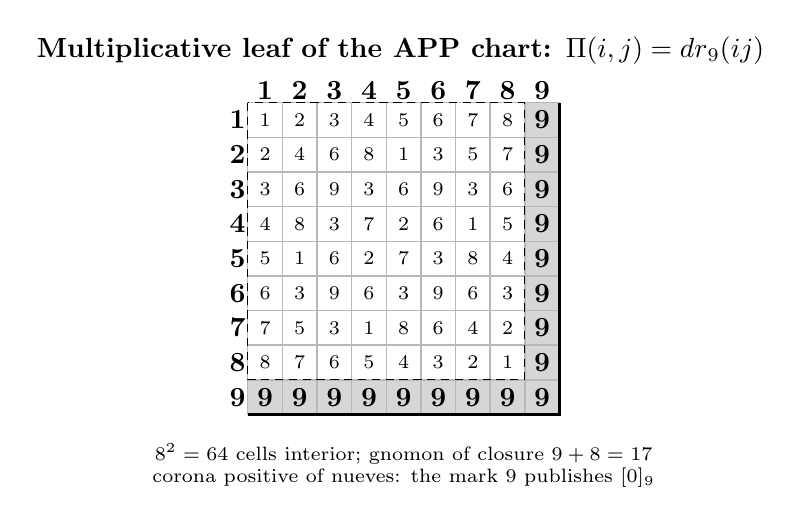
\begin{tikzpicture}[
  font=\scriptsize,
  cell/.style={minimum width=4.35mm,minimum height=4.35mm,
    inner sep=0pt,draw=black!28}]
  \node[font=\bfseries] at (1.72,.88)
    {Multiplicative leaf of the APP chart: $\Pi(i,j)=\operatorname{dr}_9(ij)$};
  \foreach \i in {1,...,9}{
    \node[font=\bfseries] at (-.35,{-(\i-1)*.44}) {\i};
    \foreach \j in {1,...,9}{
      \pgfmathtruncatemacro{\v}{mod(\i*\j-1,9)+1}
      \pgfmathtruncatemacro{\border}{(\i==9)||(\j==9)}
      \ifnum\border=1
        \node[cell,fill=black!16,font=\bfseries]
          at ({(\j-1)*.44},{-(\i-1)*.44}) {\v};
      \else
        \node[cell,fill=white]
          at ({(\j-1)*.44},{-(\i-1)*.44}) {\v};
      \fi
    }
  }
  \foreach \j in {1,...,9}{
    \node[font=\bfseries] at ({(\j-1)*.44},.38) {\j};
  }
  \draw[very thick] (3.74,.22)--(3.74,-3.74)--(-.22,-3.74);
  \draw[densely dashed] (-.22,.22) rectangle (3.30,-3.30);
  \node[align=center,anchor=north,font=\scriptsize] at (1.76,-3.98)
    {$8^2=64$ cells interior; gnomon of closure
     $9+8=17$\\corona positive of nueves: the mark $9$ publishes $[0]_9$};
\end{tikzpicture}}
\end{minipage}\hfill
\begin{minipage}[t]{.44\textwidth}
\centering
\resizebox{.98\linewidth}{!}{%
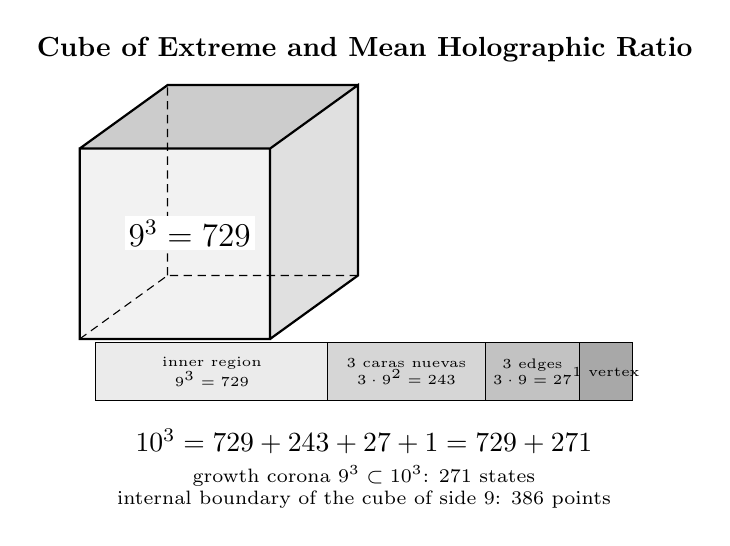
\begin{tikzpicture}[font=\scriptsize]
  \begin{scope}[x={(.78cm,0cm)},y={(.36cm,.26cm)},z={(0cm,.78cm)}]
    \coordinate (O) at (0,0,0);
    \coordinate (X) at (3.1,0,0);
    \coordinate (Y) at (0,3.1,0);
    \coordinate (XY) at (3.1,3.1,0);
    \coordinate (Z) at (0,0,3.1);
    \coordinate (XZ) at (3.1,0,3.1);
    \coordinate (YZ) at (0,3.1,3.1);
    \coordinate (XYZ) at (3.1,3.1,3.1);
    \path[fill=black!5] (O)--(X)--(XZ)--(Z)--cycle;
    \path[fill=black!12] (X)--(XY)--(XYZ)--(XZ)--cycle;
    \path[fill=black!20] (Z)--(XZ)--(XYZ)--(YZ)--cycle;
    \draw[densely dashed] (O)--(Y)--(XY) (Y)--(YZ);
    \draw[thick] (O)--(X)--(XZ)--(Z)--cycle
      (X)--(XY)--(XYZ)--(XZ) (Z)--(YZ)--(XYZ);
    \node[font=\bfseries\large,fill=white,inner sep=1.5pt]
      at (1.55,.52,1.55) {$9^3=729$};
  \end{scope}
  \node[font=\bfseries] at (3.62,3.68) {Cube of Extreme and Mean Holographic Ratio};
  \draw[fill=black!8] (0.2,-.78) rectangle (3.15,-.05);
  \node[align=center,font=\tiny] at (1.68,-.415)
    {inner region\\$9^3=729$};
  \draw[fill=black!16] (3.15,-.78) rectangle (5.15,-.05);
  \node[align=center,font=\tiny] at (4.15,-.415)
    {$3$ caras nuevas\\$3\cdot9^2=243$};
  \draw[fill=black!24] (5.15,-.78) rectangle (6.35,-.05);
  \node[align=center,font=\tiny] at (5.75,-.415)
    {$3$ edges\\$3\cdot9=27$};
  \draw[fill=black!34] (6.35,-.78) rectangle (7.02,-.05);
  \node[align=center,font=\tiny] at (6.685,-.415)
    {$1$ vertex};
  \node[font=\bfseries] at (3.61,-1.30)
    {$10^3=729+243+27+1=729+271$};
  \node[align=center] at (3.61,-1.88)
    {growth corona $9^3\subset10^3$: $271$ states\\
     internal boundary of the cube of side $9$: $386$ points};
\end{tikzpicture}}
\end{minipage}
\caption{Two finite publications of the support. Left: the product table with positive digital root and its closure gnomon. Right: the EMRH cubic completion, which distinguishes interior, faces, edges, and vertex. The growth corona $271$ and the internal boundary $386$ are two typed counts: the former measures the enlargement $9^3\subset10^3$ and the latter the boundary of the cube of side $9$.}
\label{fig:app-emrh-mini}
\end{figure}
